
% Лабораторная работа по АСиСу № 3
% Михедов Константин Константинович

% Тип документа: статья, на бумаге А4
\documentclass[a4paper]{article}

% Подключение сторонних tex файлов 
\usepackage{import}


% Основные данные - ВУЗ, факультет, город...
\import{./../../stuff/tex}{config.tex}

% Подключение необходимых зависимостей
\import{./../../stuff/tex/settings}{packages.tex}
% Настройка подключенных пакетов
\import{./../../stuff/tex/settings}{preferences.tex}


% Шаблон титульной страницы 
\import{./../../stuff/tex/templates}{title.tex}
% Упрощенный блок "выполнил"
\import{./../../stuff/tex/templates}{sign1.tex}
% Макрос для содержания
\import{./../../stuff/tex/templates}{toc.tex}

% Определяем название документа
\title{
  Лабораторная работа №4 по курсу \\
  <<Компьютерный практикум <<Админимтрирование систем и сетей>>  
}
% Отключаем отображение правительства
\renewcommand{\government}{}
% Отключаем сокращенное нзавание университета
\renewcommand{\subuniversity}{}
% Указываем преподавателя
\renewcommand{\shortteachername}{Зудин Д.Е.}


% Путь до внешних изображений
\graphicspath{ {./figures/}}


% Основной текст работы
\begin{document}
  \templatedtitlepage
  
  \toc
  \section{Ход работы}

  \subsection{Начало захвата пакетов}

  В ходе данной лабораторной работы потребуется анализировать
  трафик, для этого необходимо запустить снифер - \textit{Wireshark} (рис. \ref{img:0001} на стр. \pageref{img:0001}),
  и начать захват пакетов на используемом сетевом интерфейсе (рис. \ref{img:0002} на стр. \pageref{img:0002}).

  \begin{figure}[H]
    \centering
    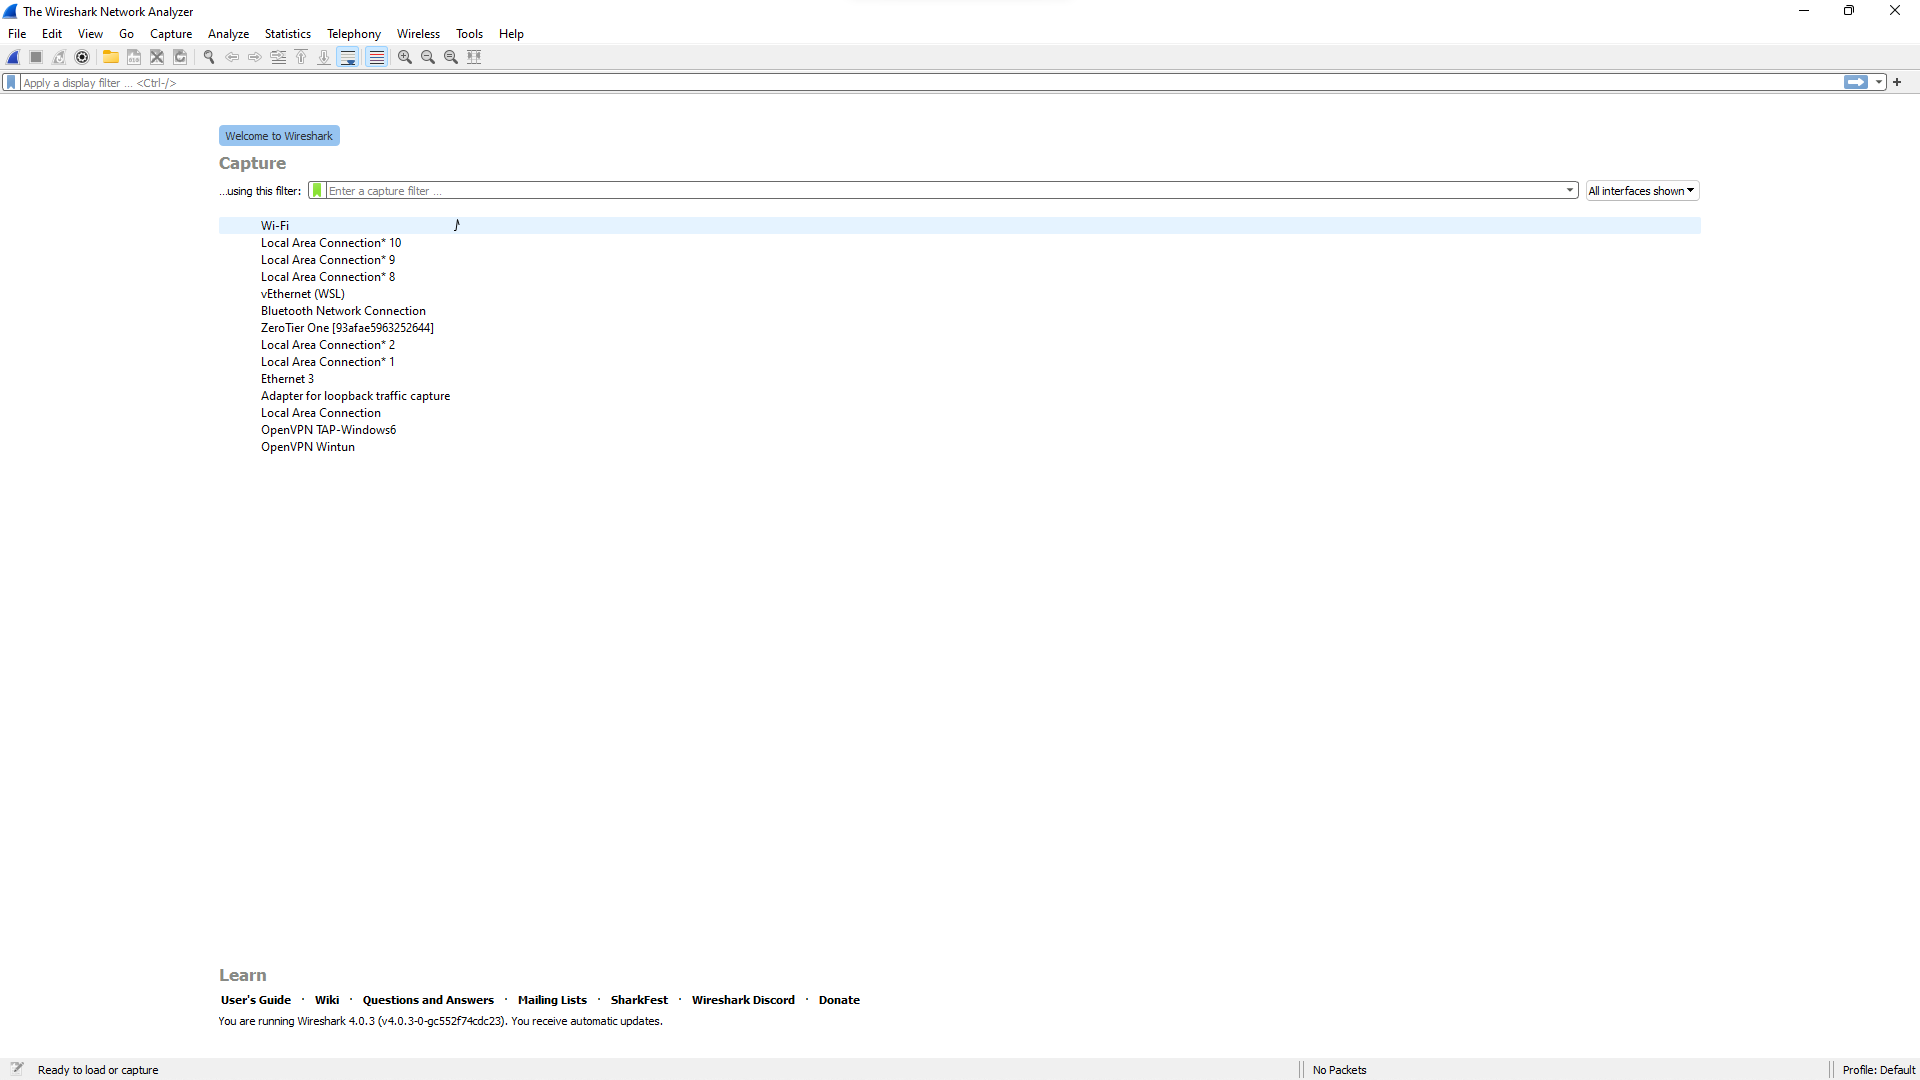
\includegraphics[width=0.8\textwidth]{04_00 (1)}
    \caption{Открываем Wireshark}
    \label{img:0001}
  \end{figure}
  
  \begin{figure}[H]
    \centering
    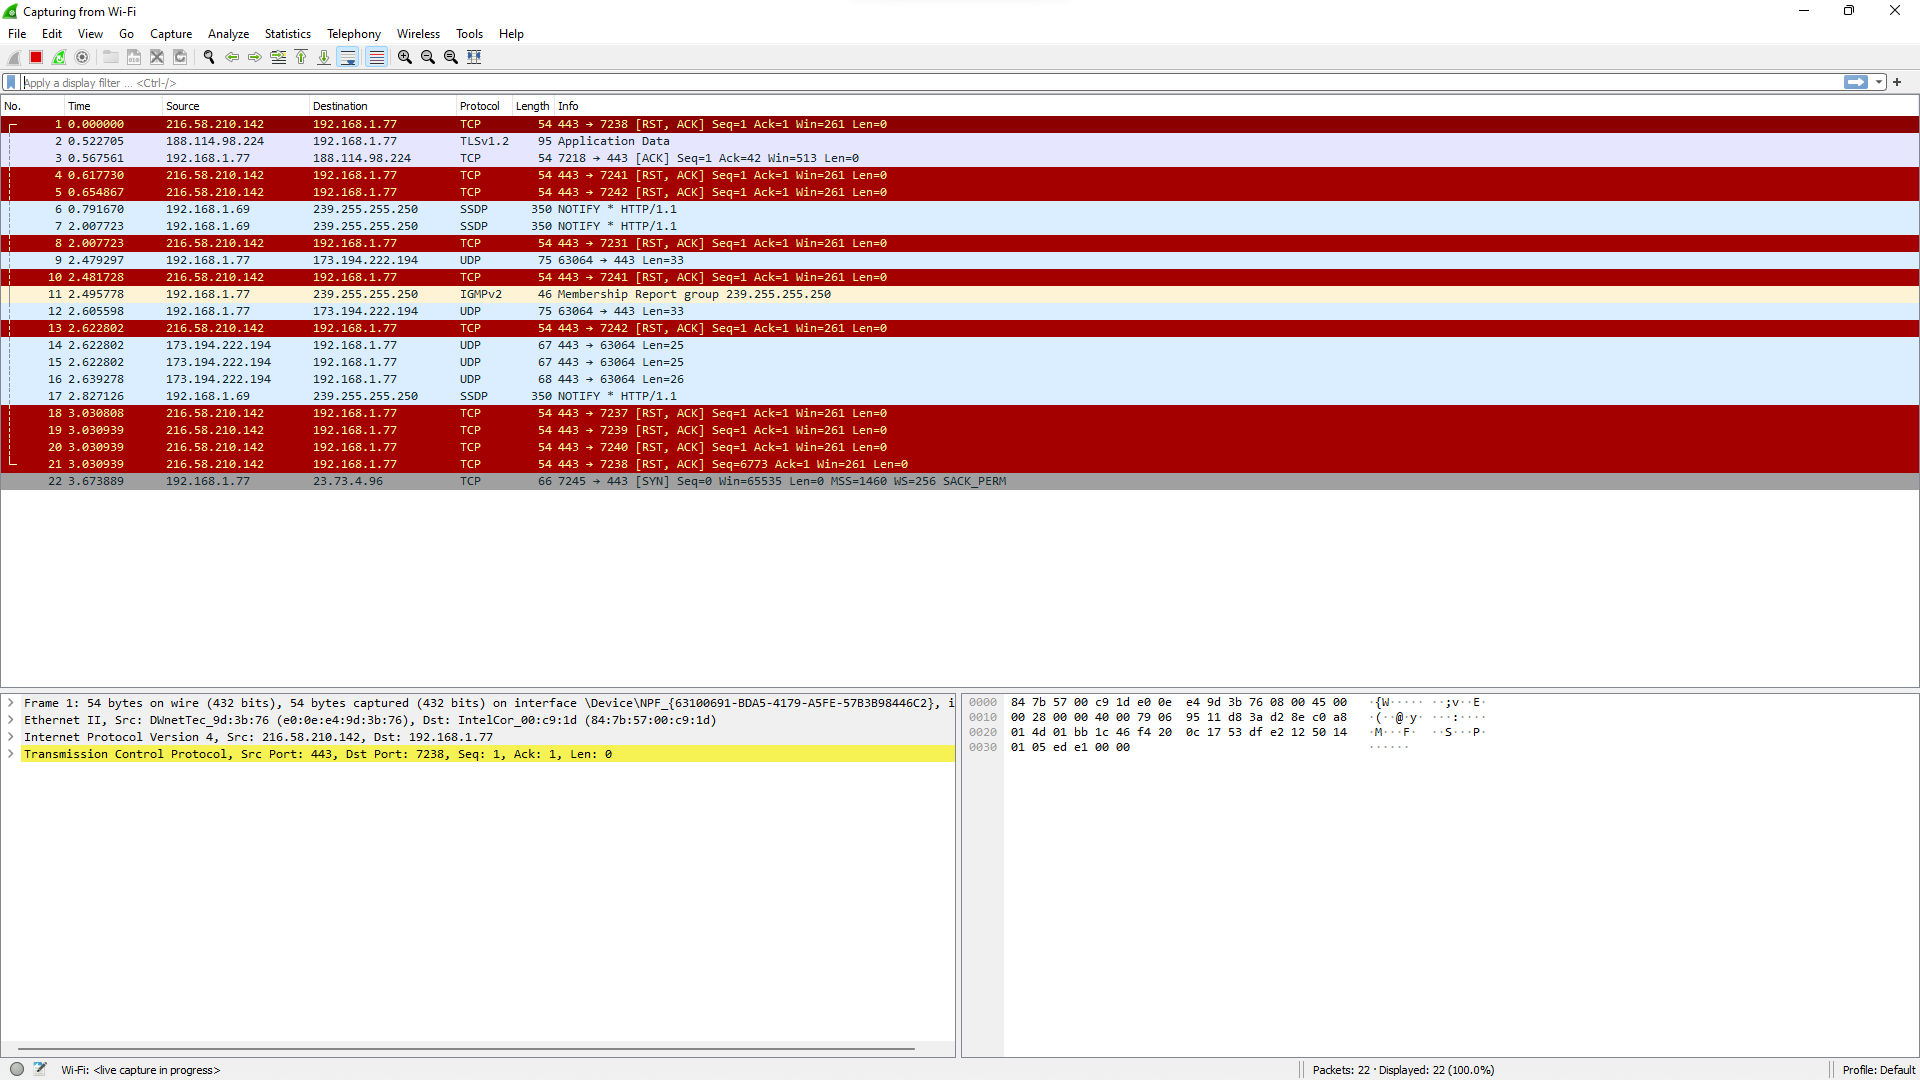
\includegraphics[width=0.8\textwidth]{04_00 (2)}
    \caption{Запущенный захват пакетов}
    \label{img:0002}
  \end{figure}

  Так как в ходе работы анализироваться будут только \textit{DHCP}-пакеты,
  можно сразу настроить пододящий фильтр (рис. \ref{img:0003} на стр. \pageref{img:0003}):

  \begin{figure}[H]
    \centering
    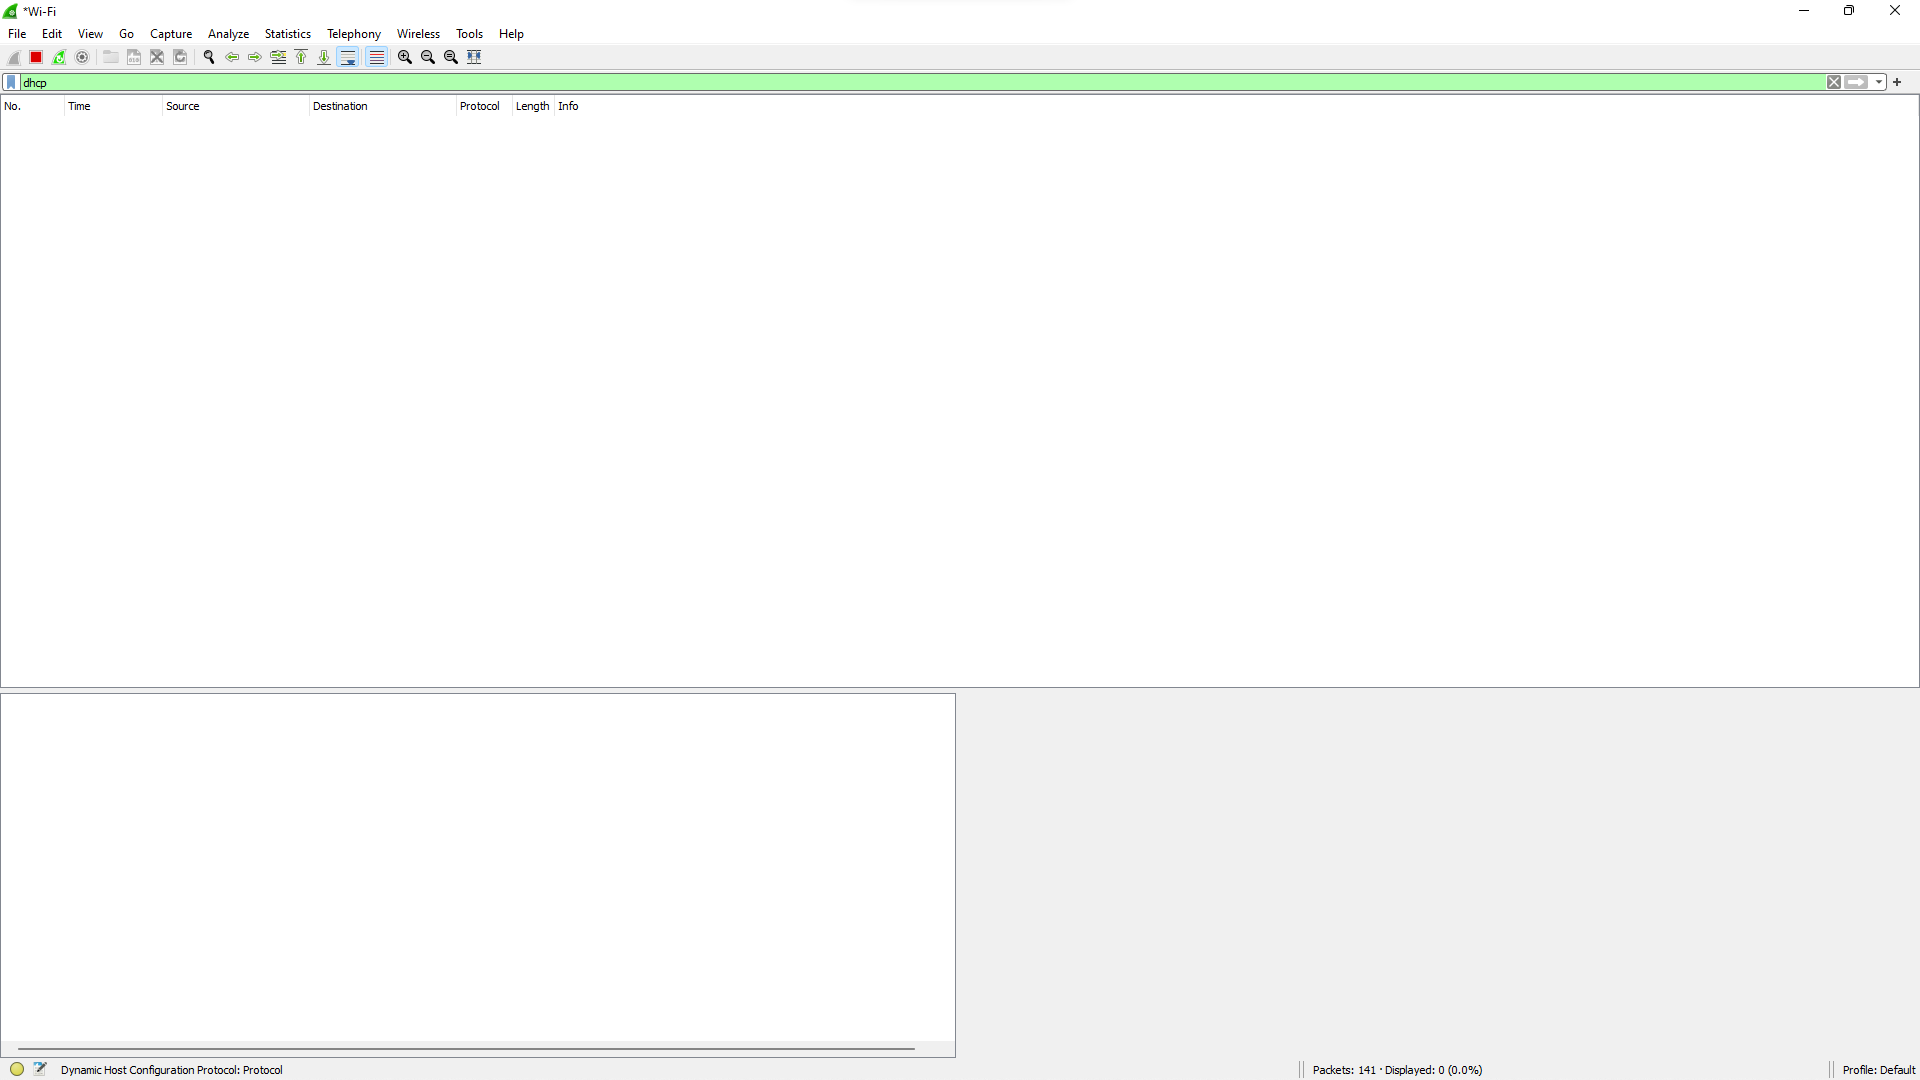
\includegraphics[width=0.8\textwidth]{04_00 (3)}
    \caption{Фильтр - отображаются только перехваченные DHCP-пакеты}
    \label{img:0003}
  \end{figure}

  \subsection{Выполнение DHCP-запросов}

  Прежде всего необходимо узнать имя сетевого интерфейса, для которого
  будут производиться последующие операции. В ОС семейства \textit{Windows}
  это можно сделать при помощи утилиты \textit{ipconfig} (рис. \ref{img:0004} на стр. \pageref{img:0004}):
  
  \begin{figure}[H]
    \centering
    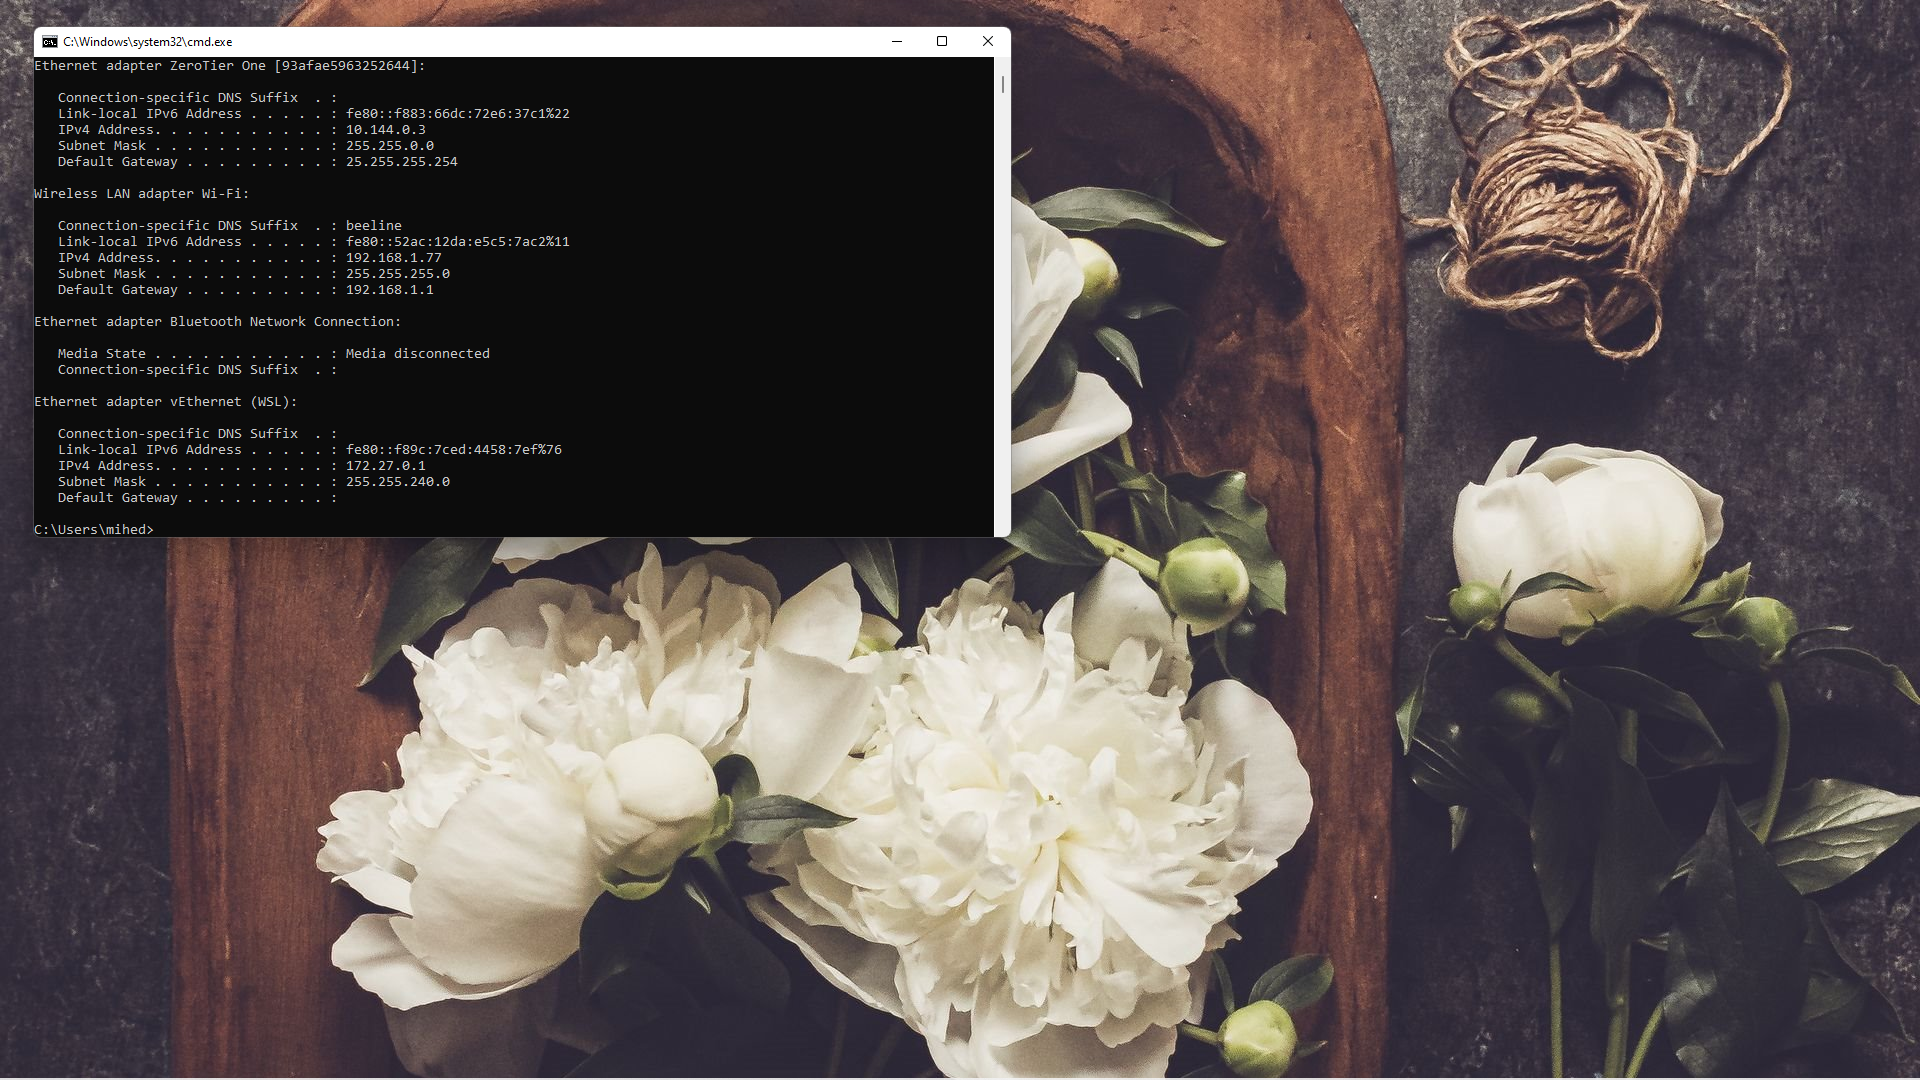
\includegraphics[width=0.8\textwidth]{04_00 (4)}
    \caption{Информация о имеющихся сетевых интерфейсах}
    \label{img:0004}
  \end{figure}

  Для выполнения запросов будет использоваться интерфейс \textbf{Wi-Fi} с
  уже назначенным \textit{IPv4} адресом - 192.168.1.77.
 Освободим полученный адрес при помощи той же утилиты (рис. \ref{img:0005} на стр. \pageref{img:0005}):

  \begin{figure}[H]
    \centering
    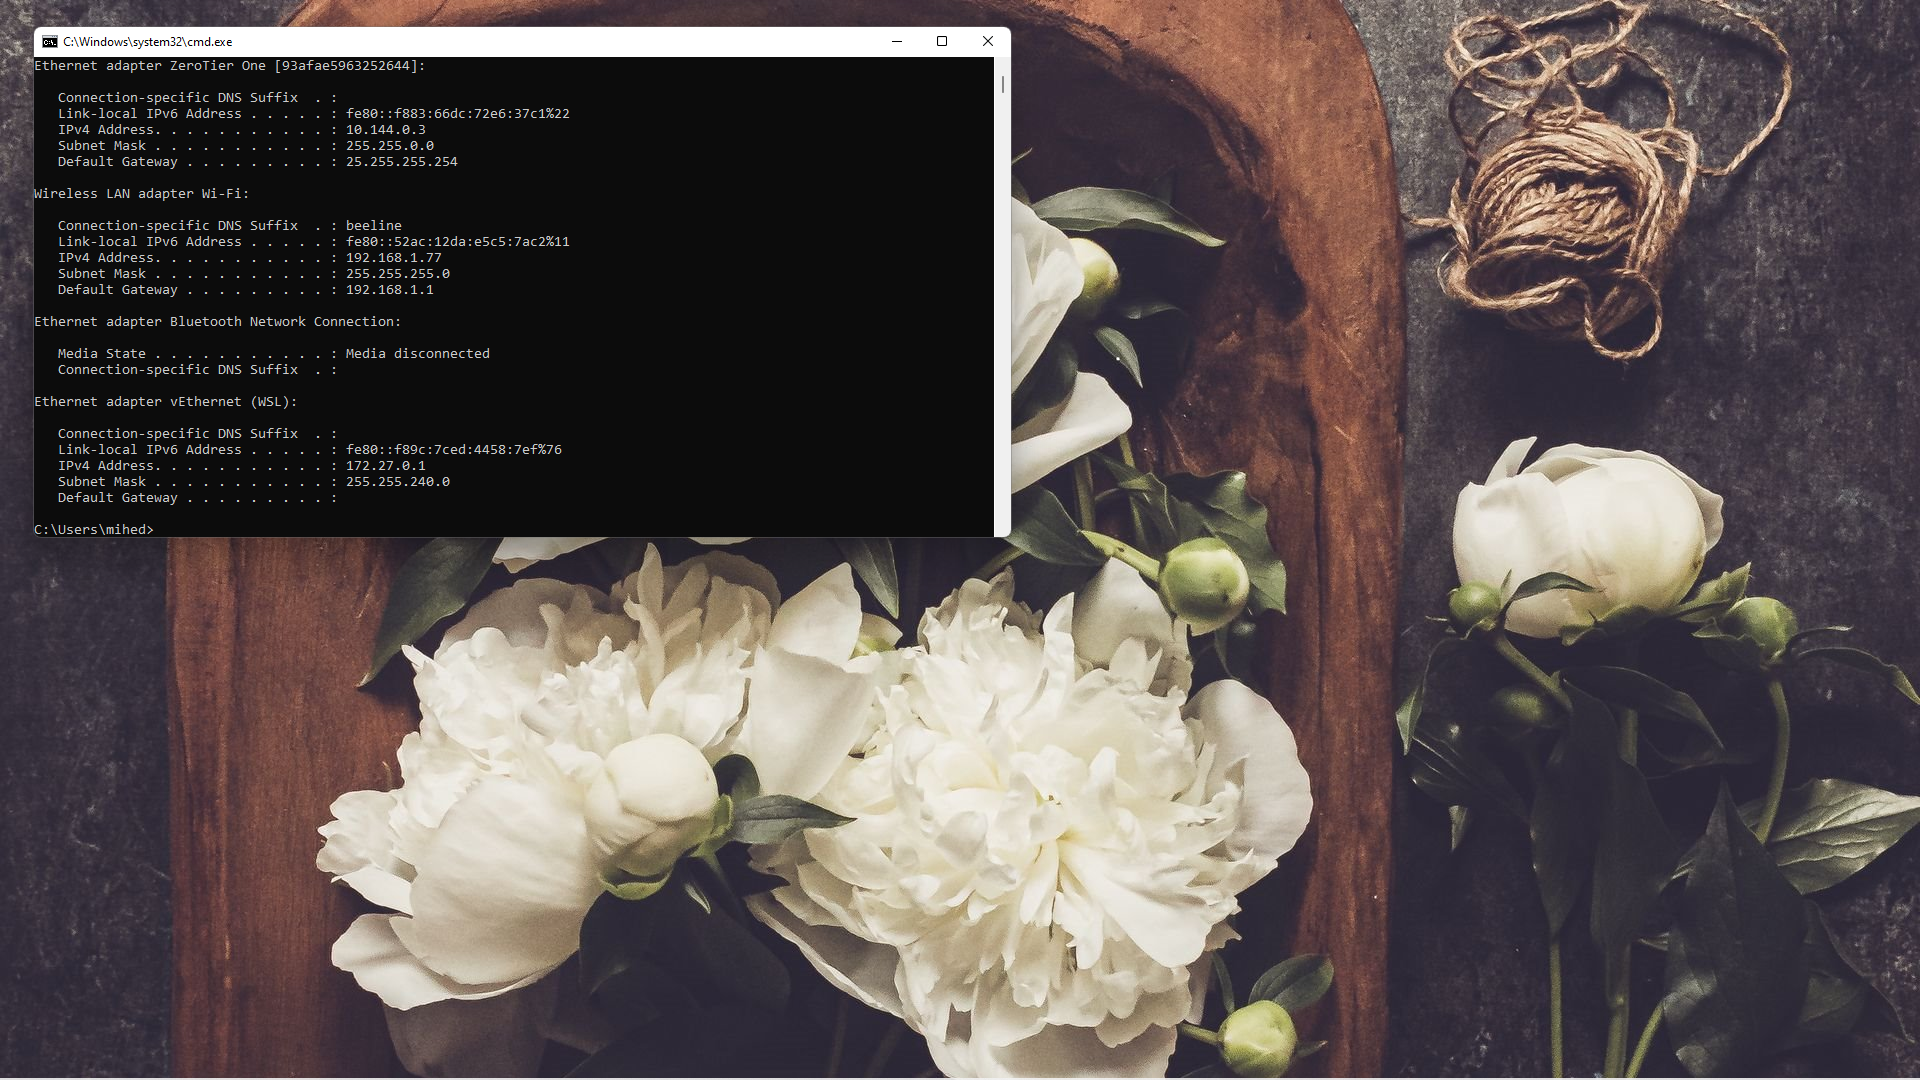
\includegraphics[width=0.8\textwidth]{04_00 (4)}
    \caption{ipconfig /release "Wi-Fi" - освобождение занятого IPv4-адреса}
    \label{img:0005}
  \end{figure}

  Можно увидеть только что отправленный \textit{DHCP RELEASE} запрос при помощи \textit{Wireshark}
  (рис. \ref{img:0006} на стр. \pageref{img:0006}):

  \begin{figure}[H]
    \centering
    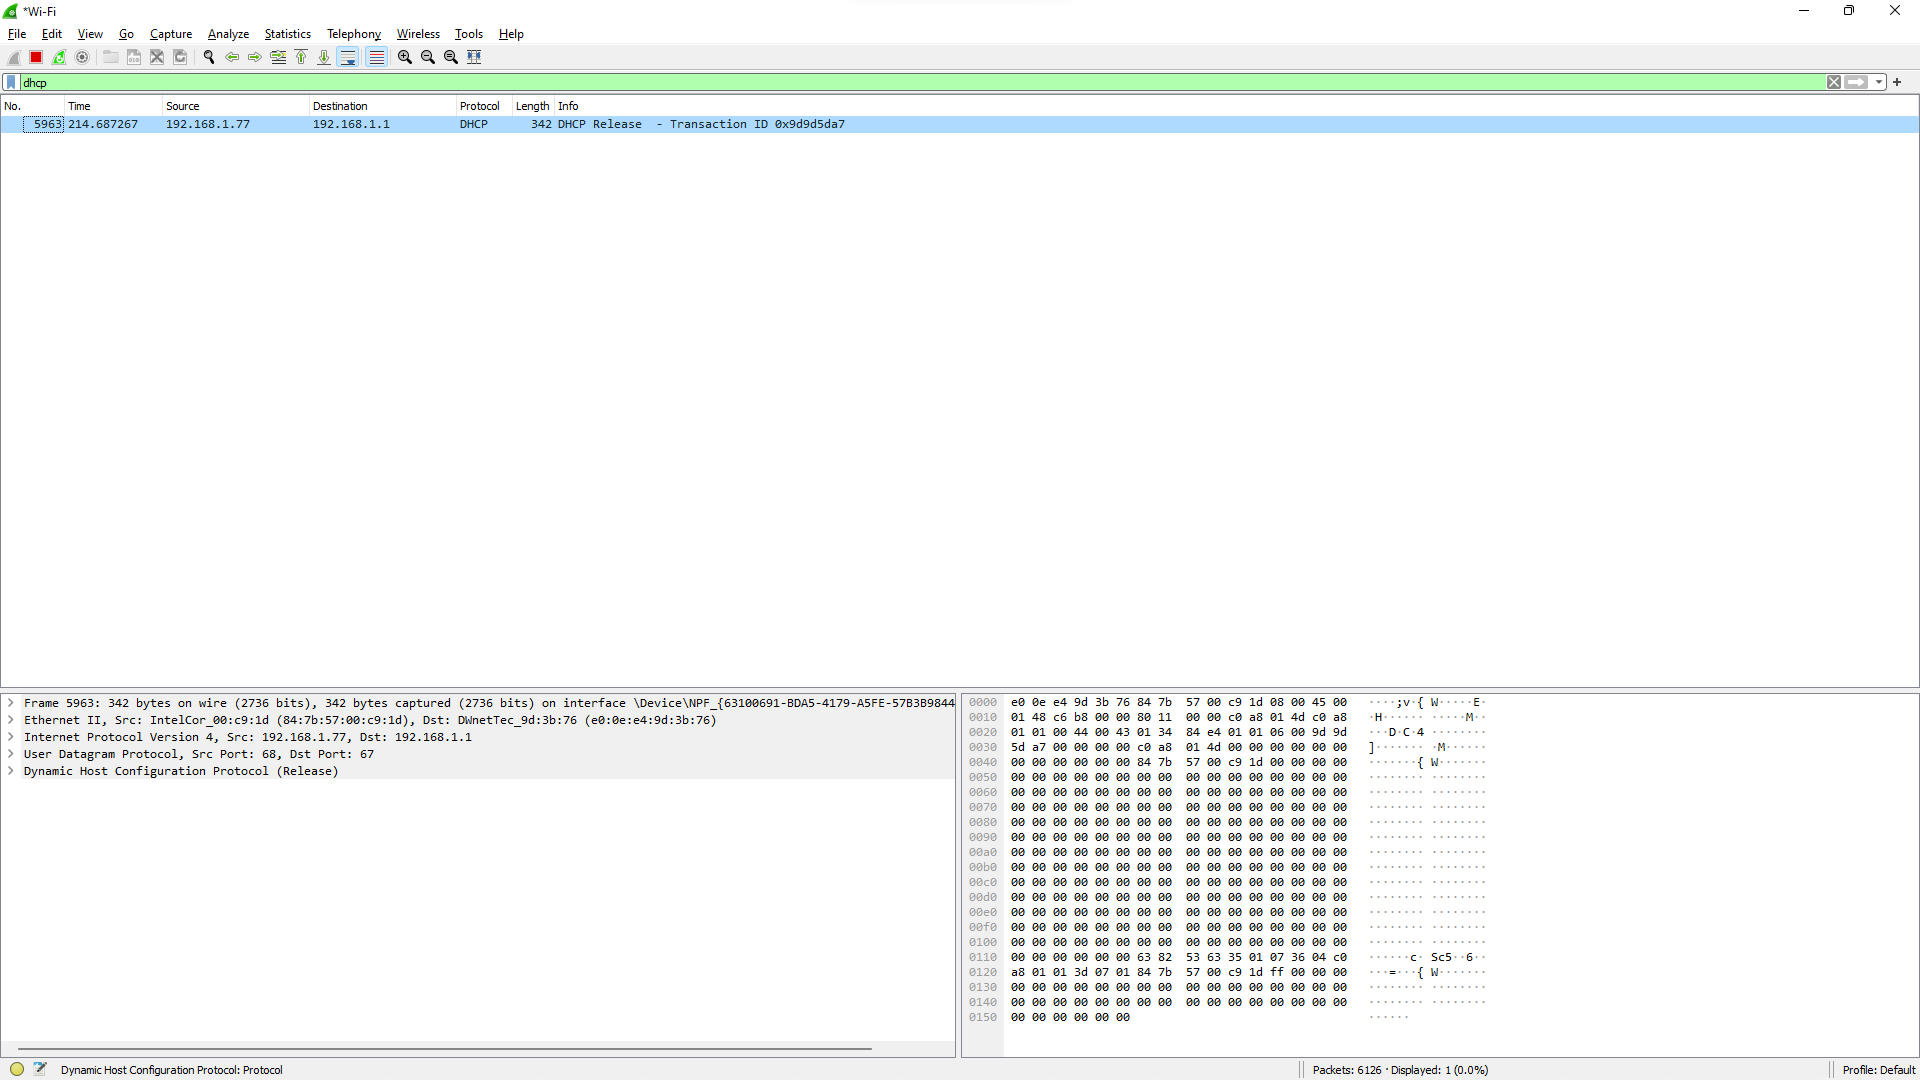
\includegraphics[width=0.8\textwidth]{04_00 (6)}
    \caption{Перехваченный RELEASE запрос}
    \label{img:0006}
  \end{figure}

  Теперь сетевой интерфейс \textbf{Wi-Fi} не имеет назначенного \textit{IP}-адреса,
  запросим новый при помощи того же \textit{ipconfig} (рис. \ref{img:0007} на стр. \pageref{img:0007}):

  \begin{figure}[H]
    \centering
    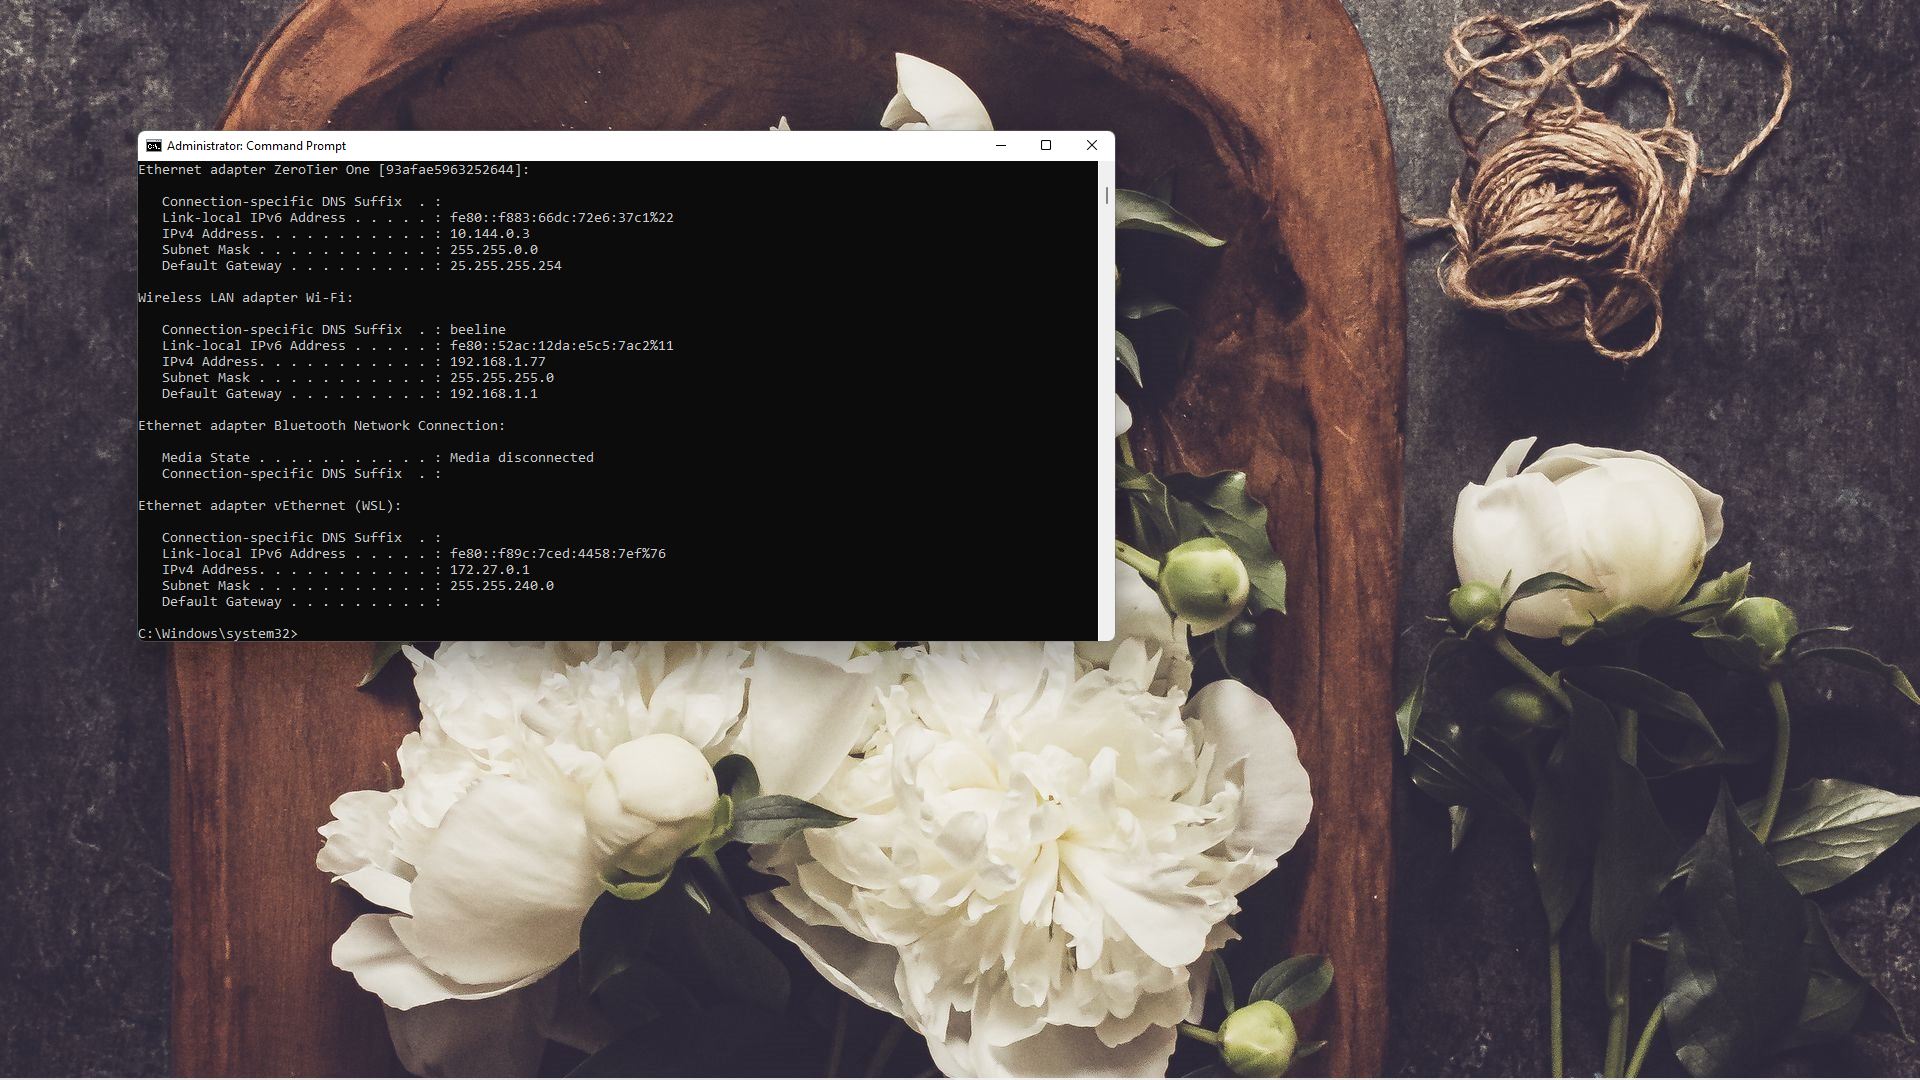
\includegraphics[width=0.8\textwidth]{04_00 (7)}
    \caption{ipconfig /renew - выполнить DNS DISCOVER запрос}
    \label{img:0007}
  \end{figure}

  Как видно из вывода утилиты - компьютеру снова был назначен адрес 192.168.1.77.

  \subsection{Анализ трафика}

  Все необходимые \textit{DHCP}-запросы были выполнены - теперь необходимо остановить
  сниффинг и проанализировать захваченные пакеты (рис. \ref{img:0008} на стр. \pageref{img:0008}):

  \begin{figure}[H]
    \centering
    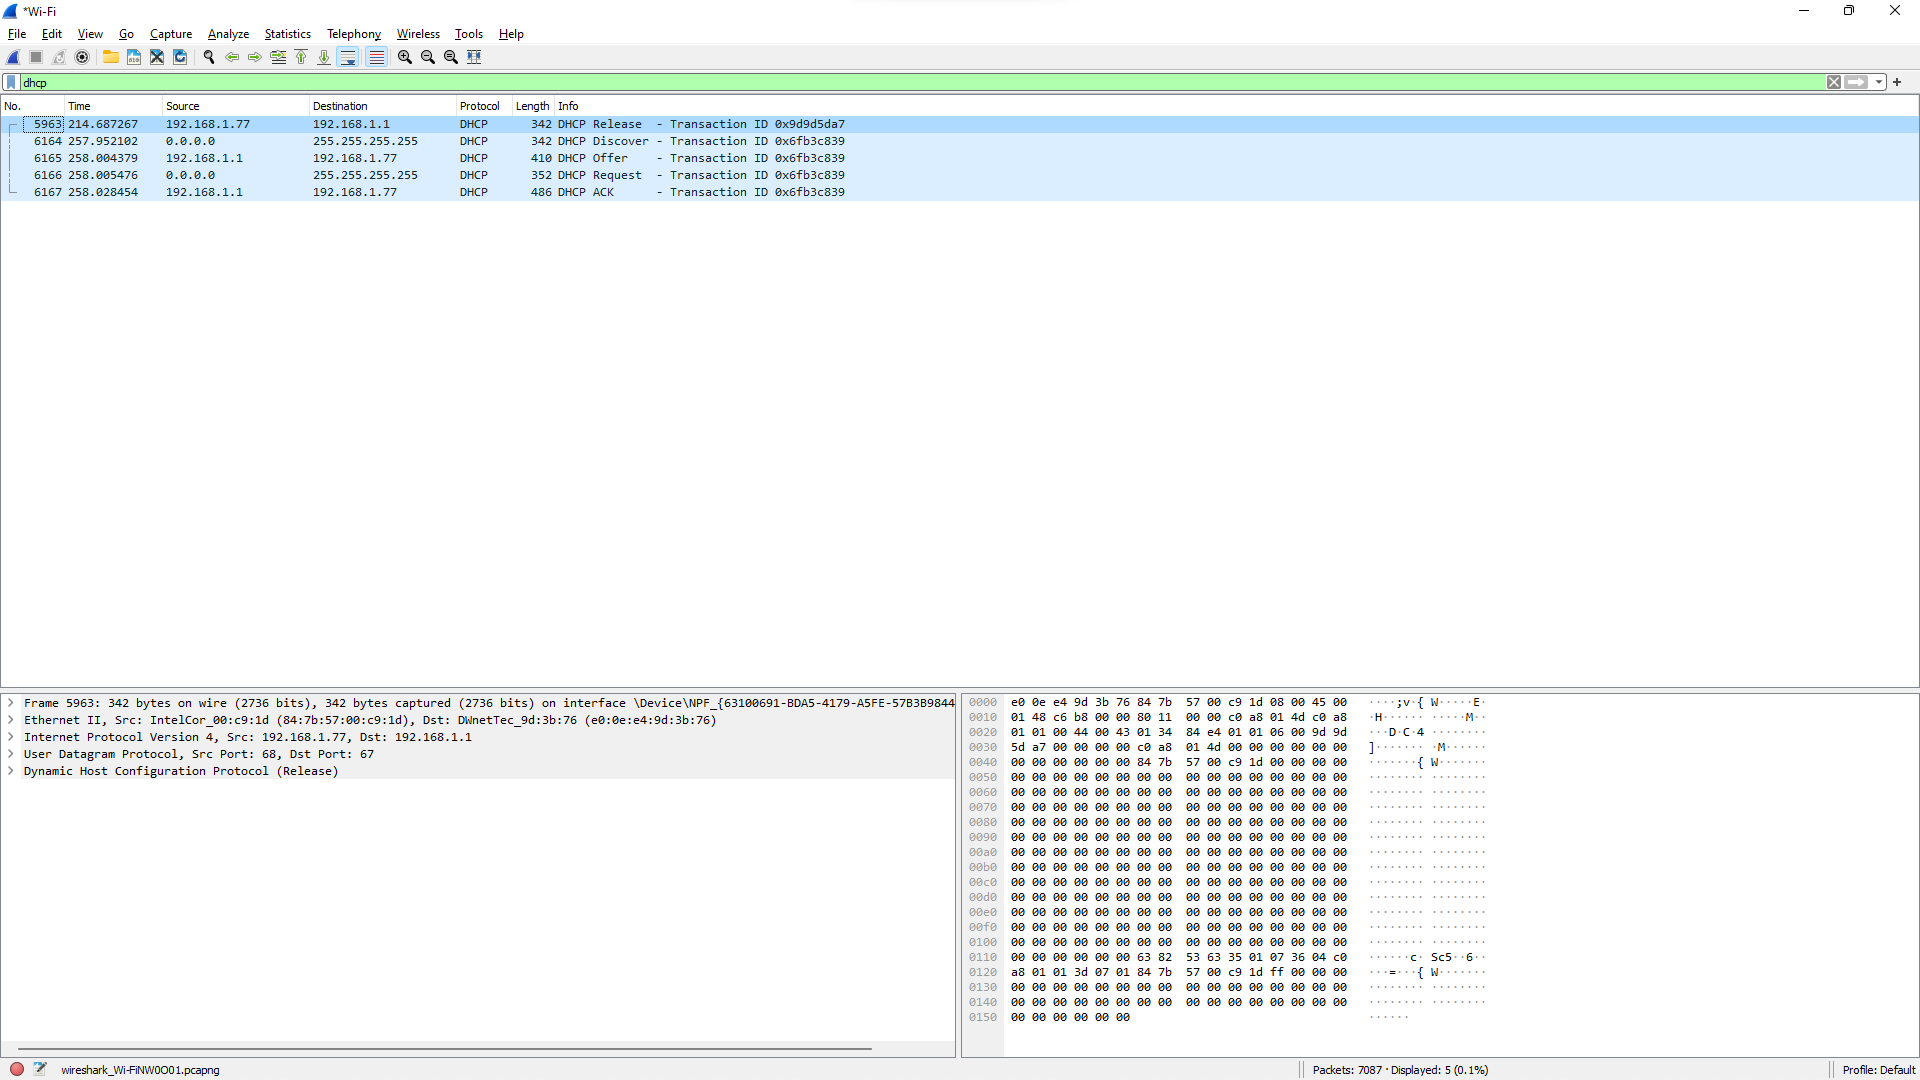
\includegraphics[width=0.8\textwidth]{04_00 (8)}
    \caption{Все перехваченные DHCP-пакеты}
    \label{img:0008}
  \end{figure}

  \textit{Wireshark} перехватил еще 4 подходящих по типу пакета (дополнительно к RELEASE запросу).
  Можно заметить, что процесс получения \textit{IP}-адреса действительно описывается
  схемой \textit{DiscoverOfferRequestAcknowledge}.

  Наибольший интерес для нас представляет \textit{DHCP Offer} - ответ \textit{DHCP}-сервера
  на наш запрос. Откроем и развернем информацию о данном пакете (рис. \ref{img:0009} на стр. \pageref{img:0009}):

  \begin{figure}[H]
    \centering
    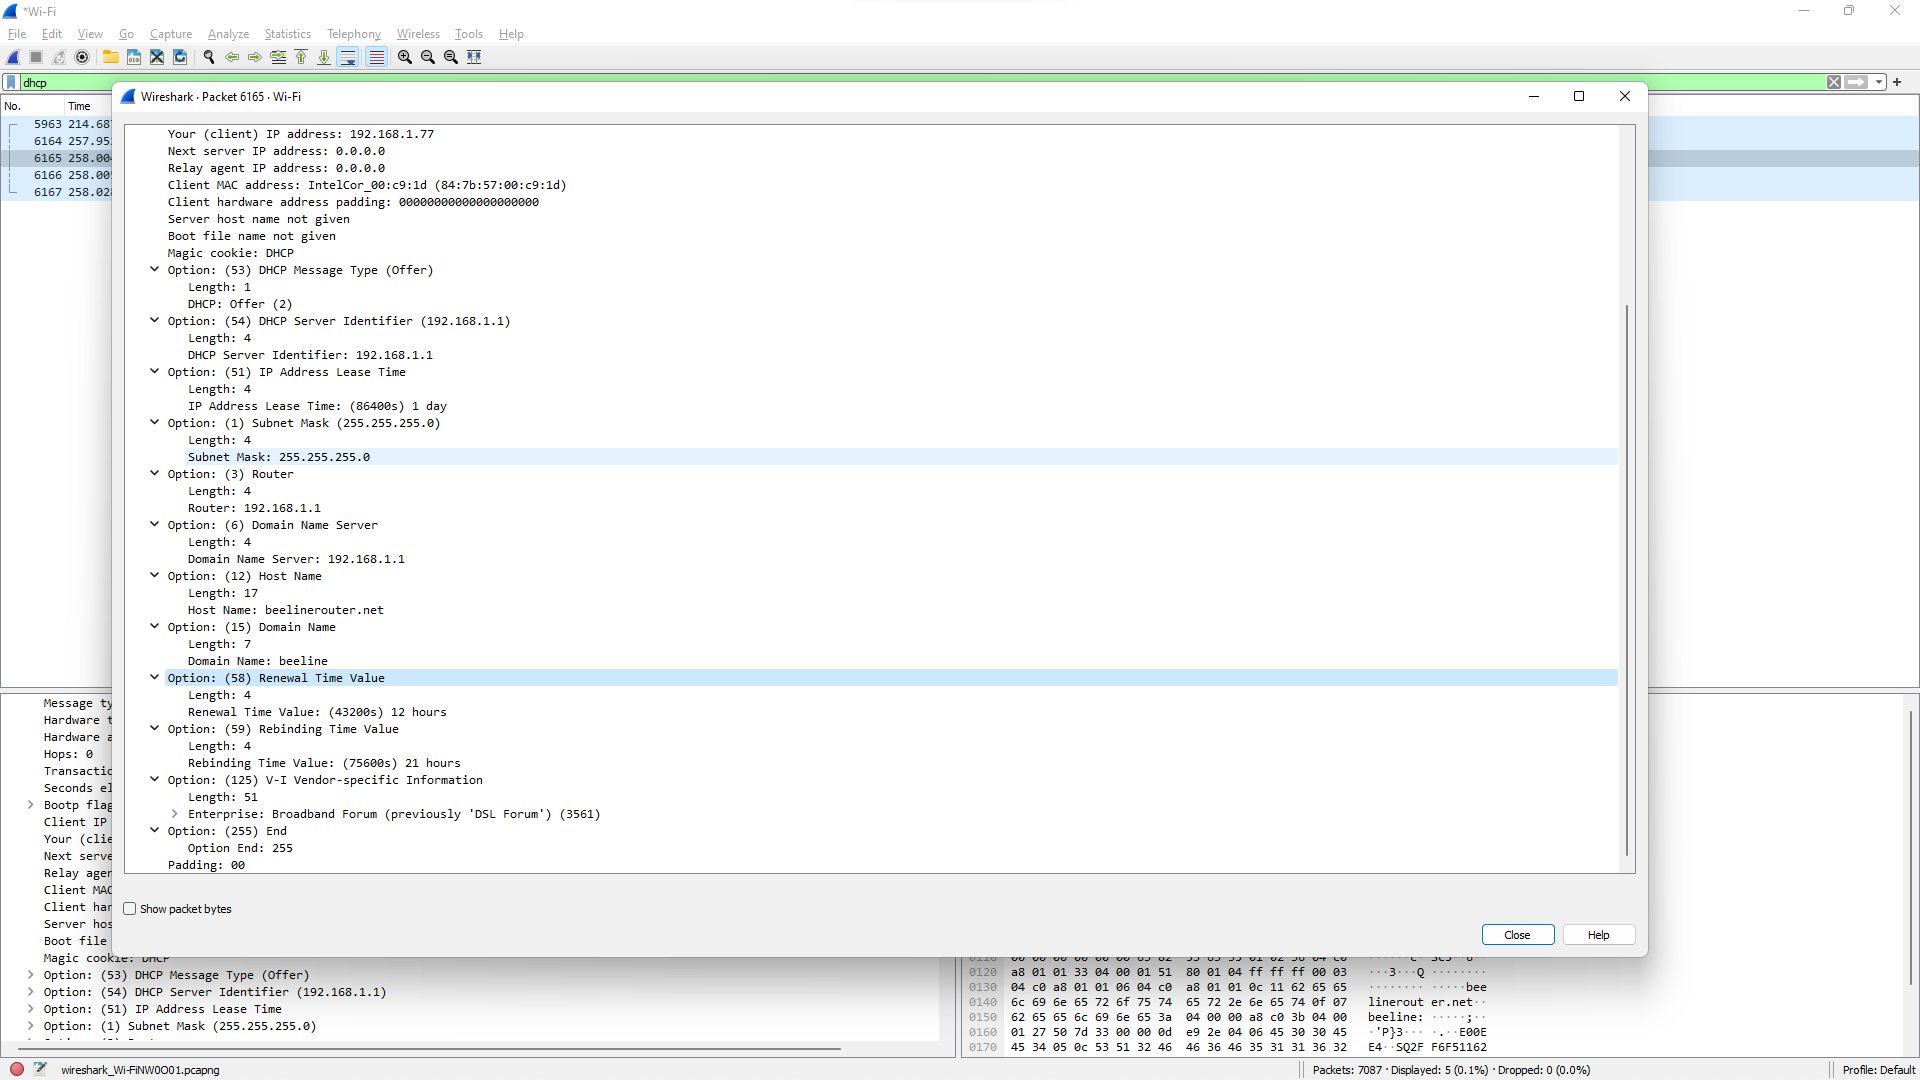
\includegraphics[width=0.8\textwidth]{04_00 (15)}
    \caption{Информация о DHCP OFFER ответе}
    \label{img:0009}
  \end{figure}

  Самое важное, что можно достать из этого запроса - информаиця о том, что клиенту
  с \textit{MAC}-адресом 84:7b:57:00:c9:1d был предложен следующий \textit{IPv4}-адрес:
  192.168.1.77 (причем предложен всего на 1 день).

  Видно, что \textit{DHCP}-пакет содержит в себе информацию о своем типе (является он 
  RELEASE, DISCOVER, OFFER, REQUEST или ACKNOWLEDGE пакетом), в данном случае - OFFER.

  Из данного пакета можно достать информацию о \textit{DHCP} сервере -
  он имеет \textit{IPv4}-адрес 192.168.1.1, имеет доменное имя - beelinerouter.net
  и собственное имя (компьютера) - beeline.

  Также в ответе содержиться маска текущей подсети - 255.255.255.0, и адрес
  \textit{DNS} сервера по умолчанию - 192.168.1.1.

  Можно также выделить, что временной инетрвал обновления \textit{IP}-адреса
  составляет 12 часов, а интервад его полного переопределения - 21 час.

  \section{Вывод}

  В ходе данной лабораторной рабоыты мной были получены навыки ручного выполнения 
  \textit{DHCP}-запросов при помощи командной строки, также удалось разобраться
  во внутренней структуре, устройстве данного протокола, проанализировать
  передаваемую им информацию.

\end{document}
